\newpage
\fancyhead[R]{\sffamily\small\color{Muted}Vulkan / 镂空材质}
\section{Sponza 的镂空材质}

在 Sponza 长廊里，花盆中的叶片画在带纹理的三角形上。贴图里透明的部分应该让光穿过。旧版判断点光源有没有被挡住时，射线一碰到叶片的三角形就可能停下。修正后，射线先读命中位置的透明度，碰到孔洞就继续向前找。直接光、探针、反射和雾都用到了这项查询。

\begin{figure}[H]\centering
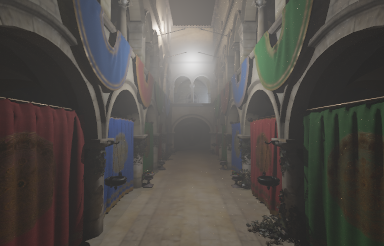
\includegraphics[width=.60\linewidth]{gi-mask/sponza-timing-view.png}
\caption{正式 Vulkan 编辑器实际计时的机位。RenderDoc 回放导出第 24 帧的面板颜色，画幅为 $384\times246$。两次捕获都开启分簇点光源、DDGI、GTAO、SSR、体积雾与 TAA。}
\end{figure}

用 RTX 5070 Ti Laptop GPU 运行 Debug x64 编辑器。保持模型、相机、灯光与渲染设置相同，在 RenderDoc 1.47 里将旧版和修正版各预热一次，再分别回放 11 次。下表记录每条计算命令在 GPU 上执行的毫秒数，取 11 次的中位数。末列为修正后减去修正前，正值表示这次测得的时间增加。

{\smalltable\noindent\begin{tabularx}{\linewidth}{@{}Xrrrr@{}}\toprule
计算命令 & 事件 & 整面遮挡 & 按贴图裁剪 & 差值（ms）\\\midrule
\maskTimingRows
\bottomrule\end{tabularx}\par}

两帧的场景和界面都合计绘制 228 次，计算命令均为 12 条。分簇点光源一行只测给表面算光的命令，前面把点光源分到各簇的时间另算。反射一行包括先查屏幕、再查场景的整个过程。表中雾的耗时最长，每条视线沿途取 8 处样本，还要检查各处能否收到灯光。

读取透明度会增加取样，光穿过小孔也会改变随后访问的三角形。这两项工作的次数目前没有分开统计。两份捕获中，点光源与雾耗时上升，探针与反射耗时下降。要分辨这些差值的来源，可以保持这套机位与设置，分别记录射线碰到几次镂空三角形、穿过了几个孔，再换几个机位核对。

\readings{\href{run:../profiling/gi-mask/sponza-timing.json}{原始帧位置、程序校验值及逐次耗时}\quad
\href{run:../../tests/replay_mask_timings.py}{回放脚本及复现命令}\\
\href{run:../profiling/gi-mask/sponza-reference.png}{同机位单帧与 256 次采样的反射参考图}\quad
\href{run:../profiling/gi-mask/sponza-reference.json}{参考图的取样记录与误差}}
